% !TeX spellcheck = en_US
% !TeX root = notes.tex
\section{Lecture 1: Bitcoin, Cryptocurrencies Blockchain Technology}
\begin{leftbar}
	Blockchain (sometimes called Distributed Ledger) is the underlying technology on top of which Bitcoin and other cryptocurrencies are built. While cryptocurrencies such as Bitcoin have been the original application, Blockcahin technology has a much wider range of applications.
\end{leftbar}
Industries to be affected by the blockchain:
\begin{itemize}
	\item Banking and Payments
	\item Cyber Security
	\item Supply Chain Management
	\item Forecasting (Research, Consulting, Analysis and Forecasting)
	\item Networking and IoT
	\item Insurance (Global Trust)
	\item Private Transport and Ride Sharing
	\item Online Data Storage
	\item Charity
	\item Voting
	\item Government
	\item Public Benefits
	\item Health Care
	\item Energy Management
	\item Online Music
	\item Retail
	\item Real Estate
	\item Crowd Funding
\end{itemize}

\subsection{Digital Cash}
Properties needed in digital cash:
\begin{itemize}
	\item Forgery (counterfeit)-proof
	\item Anonymity (at least to some extent)
	\item Cannot be spent multiple times (``Double Spend'' Problem)
\end{itemize}
\subsection{eCash}
\begin{figure}[H]
	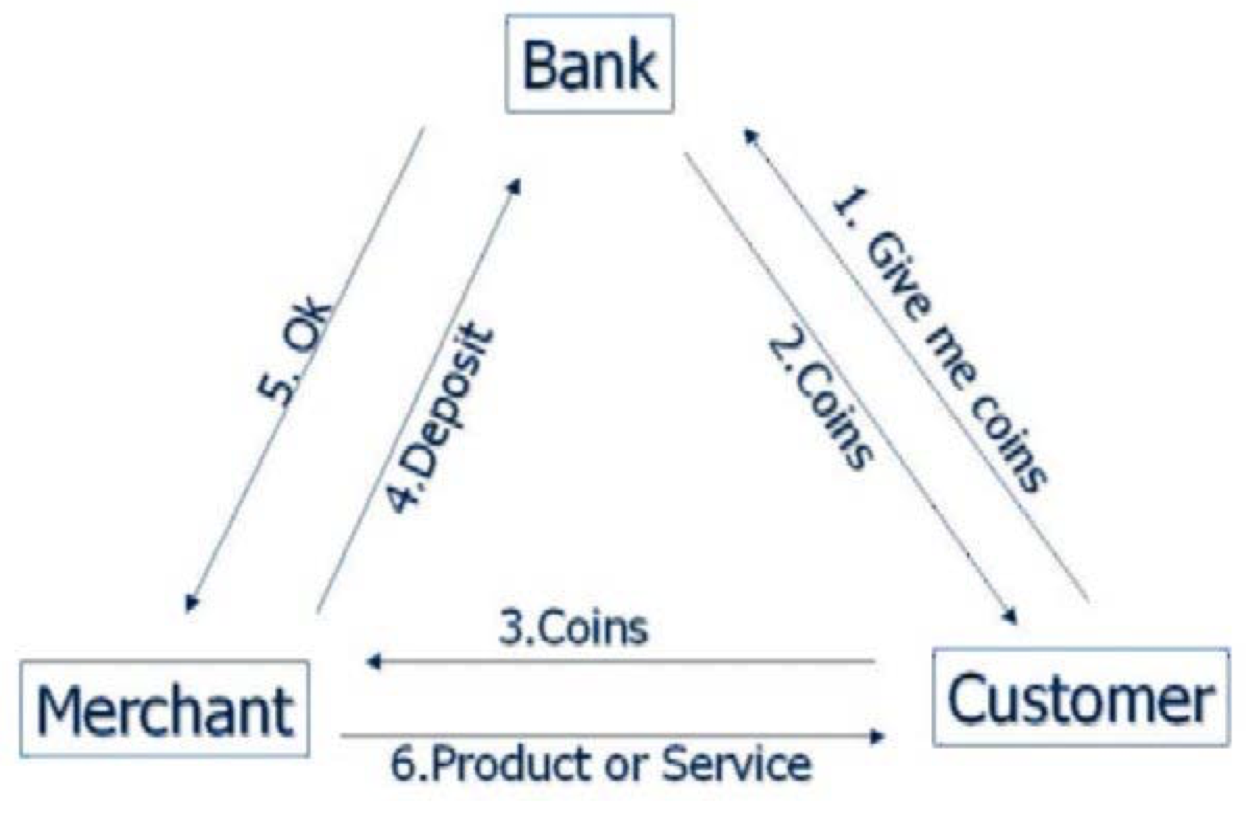
\includegraphics[width=\linewidth]{eCash}
	\centering
	\caption{eCash Step Through}
\end{figure}
\begin{itemize}
	\item eCash Transaction
	\subitem Each eCash coin has a unique identifer or ``serial number''
	\item \textbf{Forgery} can be avoided by:
	\begin{itemize}
		\item Bank digitally signing each coin
		\item Creation of valid coin requires knowing private key, everybody can verify
	\end{itemize}
	\item Avoid \textbf{Double Spending}:
	\begin{itemize}
		\item In Step 4 (Figure), bank checks if the coin has already been spent (keeps list of serial numbers of all issued and spent coins)
	\end{itemize}
	\item Provide \textbf{Anonymity}:
	\begin{itemize}
		\item You might not want the bank to know what you spend your eCash on
		\item Bank can trace coins through matching of serial numbers
		\item \textbf{Blind Signatures}
	\end{itemize}
\end{itemize}
\begin{note}{Blind Signatures}
	Signer can provide a valid digital signature without seeing what he/she is signing
\end{note}
How can Blind Signatures solve anonymity problem in eCash?
\begin{itemize}
	\item Customer creates a random serial number (sufficiently large to avoid collisions)
	\item Sends `blinded' serial number to bank
	\item Bank uses blind signature algorithm to issue a valid coin for this serial number and for the required amount, and deducts amount from user's account
	\item Customer can then `unblind' the signature, and spend valid coin at merchant
	\item Merchant sends coin to bank for checking
	\item Bank checks that it is a valid coin (valid signature), and has not been spent yet, based on serial number, and adds serial number to its `spent' list
	\item Important: \textbf{Bank cannot link serial number in coin to the customer to whom it was issued!}
\end{itemize}
\begin{note}{Bitcoin Crypto Building Blocks}
	\begin{itemize}
		\item Cryptographic Hash Functions
		\item Hash Pointers, Blockchain
		\item Merkle Trees
		\item Proof of Work methods, ``Hashcash''
		\item Digital Signatures
	\end{itemize}
\end{note}

\section{Cryptographic (one-way) Hash Function}
\begin{itemize}
	\item Also called: digital fingerprint, message digest
	\item Compact way to remember what files or blocks of data we have seen
	\item If two files have the same hash, we can be confident that they are the same
\end{itemize}
Properties of a hash function:
\begin{description}
	\item[Compression:] ``Any size'' input, fixed size output
	\item[`Easy', ``efficient'' to compute]
	\item[One-way property:] For $y=h(x)$, it is `computationally infeasible' to find $x$. Also called `pre-image resistance'
	\item[Collision resistance:] It is computationally infeasible to find any two distinct inputs $x_1$ and $x_2$ so that $h(x_1)=h(x_2)$ (Collisions do exist, actually there is an infinite number of them)
\end{description}

\subsection{Ideal One-way Cryptographic Hash Function ``Random Oracle'' Model}
\begin{itemize}
	\item A machine with an input and an output
	\item When an input arrives, if the input has arrived before $\rightarrow$ give same output as last time. Else generate a new random output and record the input and output
	\item Best approach to get specific output is brute forcing
\end{itemize}

\begin{note}{Hash Pointer}
	\begin{itemize}
		\item Points to a block of data (e.g. via an address), like a normal pointer
		\item In addition, it also stores a hash $h()$ of the data
		\item With $h()$ we can check the \textbf{integrity} of the data (i.e. if modified)
	\end{itemize}
\end{note}